\documentclass[aspectratio=169,11pt, xcolor={table}]{beamer}

%\documentclass[11pt]{beamer}

\usetheme[outer/progressbar=foot]{metropolis}


%\usepackage{tabularx}
\usepackage{booktabs}

\usepackage{gensymb}

\usepackage{siunitx}
\DeclareSIUnit \pixel{px}
\DeclareSIUnit \bit{b}

\usepackage{caption}

\usepackage{pgfplots}

%Drawing
\usepackage{tikz}

%\usepackage{tikz-3dplot}
\usetikzlibrary{shapes.geometric, shapes.misc, arrows}
\usetikzlibrary{positioning}
%\usetikzlibrary{patterns}
%\usetikzlibrary{automata}
\usepackage[europeanresistors]{circuitikz}

\newcommand{\nodeDist}{1cm}
\newcommand{\blockWidth}{1.5*\nodeDist}
\newcommand{\blockHeight}{1.5*\nodeDist}
\newcommand{\tikzStateNodeDist}{3*\nodeDist}

\tikzset{font={\small}} %set small font

\tikzstyle{block} = [rectangle, rounded corners, minimum width=\blockWidth, minimum height=\blockHeight, text centered, draw=black, fill=mLightBrown]


\tikzstyle{arrowNml} = [thick,->,>=stealth]

\tikzstyle{arrowRev} = [thick,<-,>=stealth]

\tikzstyle{arrowDbl} = [thick,<->,>=stealth]

\tikzstyle{lineNml} = [thick]



%Tables (and long tables)

\usepackage{longtable}


% alternate rowcolors for all long-tables


\let\oldlongtable\longtable


\let\endoldlongtable\endlongtable


\renewenvironment{longtable}{\rowcolors{2}{white}{mLightBrown!50}\oldlongtable} {

	
	\endoldlongtable}

%Columns example:
%	\begin{columns}
%		\begin{column}{.49\textwidth}
%		\end{column}
%	\end{columns}

\title{\huge Mercury Delay Line Emulation:\\Reconstructing Memory for EDSAC}
\date{August 30 2017}
\author{{\large Joshua Tyler}}
\begin{document}
\maketitle

\begin{frame}{What is EDSAC?}
	\centering
	\includegraphics[height=0.8\textheight]{figs/wilkes_renwick_edsac_crop}
\end{frame}


\begin{frame}{How did memory work in EDSAC?}
	\begin{columns}
	\begin{column}{.49\textwidth}
		\centering
		\includegraphics[height=0.8\textheight]{figs/delay_lines}
	\end{column}
	\begin{column}{.49\textwidth}
		\centering
		
		\begin{tikzpicture}[node distance=\nodeDist, every node/.style={transform shape}]

		
		
		\node (delay) [block, anchor=south west, minimum width=5*\nodeDist] at (0,0) {Delay Unit};

		
		\node (gate) [block, below=of delay.south west, anchor=north west] {Gate};

		
		\node (amp) [block, below=of delay.south east, anchor=north east] {Amplifier};

		
		\draw [arrowNml] (gate.west) -- ++(-0.5*\nodeDist,0) |- (delay.west);

		
		\draw [arrowNml] (delay.east) -- ++(0.5*\nodeDist,0) |- (amp.east);

		
		\draw [arrowNml] ([yshift=0.25*\nodeDist] amp.west) -- ([yshift=0.25*\nodeDist] gate.east);

		
		\draw [arrowRev] ([yshift=-0.25*\nodeDist] gate.east) -- ++(\nodeDist,0) -- ++(0,-\nodeDist) -- ++(-0.5*\nodeDist,0) node[left] {Clock Pulses};

		
		
		\end{tikzpicture}
	\end{column}
\end{columns}
\end{frame}


\begin{frame}{Reconstruction Effort}
	\centering
	\includegraphics[height=0.8\textheight]{figs/edsac_reconstructed}
\end{frame}

\begin{frame}{Reconstruction Effort}
	\centering
	\includegraphics[height=0.8\textheight]{figs/nickel-delay}
\end{frame}

\begin{frame}{Where I come in}

\begin{itemize}
	\item \alert{If you're going to cheat -- cheat big!}
	
	\item Using modern technology to create delay lines for EDSAC as close to the original as possible in terms of:
	\begin{itemize}
		\item Form
		\item Function
		\item Electrical interface
		\begin{itemize}
			\item N.B. This includes being `phantom powered'
		\end{itemize}
	\end{itemize}
	\item Creation of a test harness which can emulate the memory interface of EDSAC
\end{itemize}
\end{frame}

\begin{frame}{Literature}

	\centering
	%Trim = {left lower right upper}
	\includegraphics[trim={0 9cm 0 0.5cm},clip, height=0.8\textheight]{figs/literature}

\end{frame}

\begin{frame}{Specification}
\newcommand{\nominalLongTubeDelayMs}{1.15}
\newcommand{\maxJitterPlusSkewNs}{50} %Maximum jitter plus skew in nano seconds

\newcommand{\maxDelayInputV}{35}

\newcommand{\minDelayInputV}{25}

\newcommand{\maxDelayOutputmV}{100}

\newcommand{\minDelayOutputmV}{10}
\newcommand{\tubeLenCm}{165.5} %Tube length in cm

\newcommand{\tubeOdCm}{4.44} %Tube outer diameter in cm

\newcounter{specNo}
\tiny
\begin{longtable}{r  >{\raggedright}p{0.45\textwidth}  >{\raggedright}p{0.45\textwidth} }
	\tabularnewline
	\toprule

	
	\bfseries Item & \bfseries Specification & \bfseries Justification \tabularnewline

	
	\midrule

	
	\endhead %Everything above this will be repeated on every page

	
	\bottomrule

	
	\endfoot

	
	
	\refstepcounter{specNo}\thespecNo\label{itm:spec-delay} & \textbf{Must} be capable of producing a delayed copy of the EDSAC pulse train presented to it's input & This is the primary function of the device. \tabularnewline

	
	\refstepcounter{specNo}\thespecNo\label{itm:spec-power} & \textbf{Must} be powered from the input signal driven by EDSAC, with only minimal non-intrusive modifications made to EDSAC. & The goal of the device is to faithfully recreate the appearance and electrical interface of EDSAC, and thus large modifications such as power supply wires must be avoided. \tabularnewline

	
	\refstepcounter{specNo}\thespecNo\label{itm:spec-output-delay} & \textbf{Must} be able to have a nominal delay of \SI{\nominalLongTubeDelayMs}{\milli\second}, adjustable by at least $\pm 10\%$. & \SI{\nominalLongTubeDelayMs}{\milli\second} is the nominal delay of a long tube, as discussed in the report. An adjustable delay allows synchronisation with the system clock, with may vary. \tabularnewline


	
	\refstepcounter{specNo}\thespecNo\label{itm:spec-skew-jitter} & \textbf{Must} have a maximum per burst deviation from the nominal delay of \SI{\maxJitterPlusSkewNs}{\nano\second}. & This ensures that the delay line output will be able to synchronise with the clock of EDSAC. \SI{\maxJitterPlusSkewNs}{\nano\second} is the maximum deviation derived in the report \tabularnewline

	
	\refstepcounter{specNo}\thespecNo\label{itm:spec-skew-input-v} & \textbf{Must} be able to interface with input waveforms AC coupled bursts of \SI{13.5}{\mega\hertz} carrier, with peak voltages in the range of \SI{\minDelayInputV}{\volt} to \SI{\maxDelayInputV}{\volt}. & This is necessary to mimic the performance of the original delay line, \SI{\minDelayInputV}{\volt} to \SI{\maxDelayInputV}{\volt} is the range derived in the report. \tabularnewline

	
	\refstepcounter{specNo}\thespecNo\label{itm:spec-skew-output-v} & \textbf{Must} be able to have an adjustable nominal output voltage in the range of \SI{\minDelayOutputmV}{\milli\volt} to \SI{\maxDelayOutputmV}{\milli\volt} (peak to peak), driving into \SI{70}{\ohm}. & An adjustable output voltage in this range allows compatibility with both the original electrical interface, and that used by the reconstruction effort, \SI{\minDelayOutputmV}{\milli\volt} to \SI{\maxDelayOutputmV}{\milli\volt} is the range derived in the report. \tabularnewline

	
	\refstepcounter{specNo}\thespecNo\label{itm:spec-phys-size} & \textbf{Must} be encapsulated in a metal tube of \SI{\tubeOdCm}{\centi\metre} outer diameter, and \SI{\tubeLenCm}{\centi\metre} length. & This diameter allows the design to have the same appearance of the main memory store tubes of the original EDSAC design, the width and diameter are discussed in the report \tabularnewline

	
	\refstepcounter{specNo}\thespecNo\label{itm:spec-testing} & \textbf{Must} be accompanied by a testing device capable of emulating the signals produced by EDSAC. & This allows the delay line to be tested separately to the reconstruction project. \tabularnewline

	
	
\end{longtable}

\end{frame}

\begin{frame}{What I've done -- FPGA delay line}
	\centering
	\begin{tikzpicture}[node distance=\nodeDist, scale=0.8, every node/.style={transform shape}]
	
	\node (sync) [block, anchor=west] at (0,0) {\shortstack{Synchroniser}};
	
	\node (edge) [block, right=of sync.east, anchor=west] {\shortstack{Edge\\Detector}};
	
	\node (adder) [block, below=of edge.south, anchor=north] {\shortstack{Adder}};
	
	\node (fifo) [block, right=of adder.south east, anchor=south west, minimum height=(2*\blockHeight+\nodeDist)] {\shortstack{FIFO}};
	
	\node (comparator) [block, right=of fifo.east, anchor=west, minimum height=(2*\blockHeight+\nodeDist)] {\shortstack{Comparator}};
	
	\node (pulse) [block, right=of comparator.east, anchor=west] {\shortstack{Pulse\\Generator}};
	
	\node (ctr) [block, below=of fifo.south, anchor=north] {\shortstack{Counter}};
	
	\draw [arrowRev] (sync.west) -- node[above] {Input} ++(-1.5*\nodeDist,0);
	
	\draw [arrowNml] (sync) -- (edge);
	
	\draw [arrowNml] (edge.east) -- node[above] {\shortstack{Write\\EN}} ++(\nodeDist,0);
	
	\draw [arrowNml] (adder.east) -- node[above] {\shortstack{Write\\Data}} ++(\nodeDist,0);
	
	\draw [arrowNml] (ctr.north) -- ++(0, 0.5*\nodeDist) coordinate (ctrTop) -| (adder.south);
	
	\node[above] at (ctrTop) {Count};
	
	\draw [arrowRev] (adder.west) -- ++(-\nodeDist,0) node[left] {Delay constant};
	
	\draw [arrowNml] (ctrTop) -- ++(\nodeDist,0) |- ([yshift=0.5*\blockHeight] comparator.south west);
	
	\draw [arrowDbl] ([yshift=-0.5*\blockHeight] fifo.north east) -- node[above] {\shortstack{Read\\Port}} ([yshift=-0.5*\blockHeight] comparator.north west);
	
	\draw [arrowNml] (comparator) -- node[above] {\shortstack{EN}} (pulse);
	
	\draw [arrowNml] (pulse.east) -- node[above] {Output} ++(1.5*\nodeDist,0);
	
	\end{tikzpicture}
\end{frame}

\begin{frame}{What I've done -- Analogue interface}
	\centering
	\includegraphics[height=0.8\textheight]{figs/analogue}
\end{frame}

\begin{frame}{What I've done -- Phantom power}
	\centering
	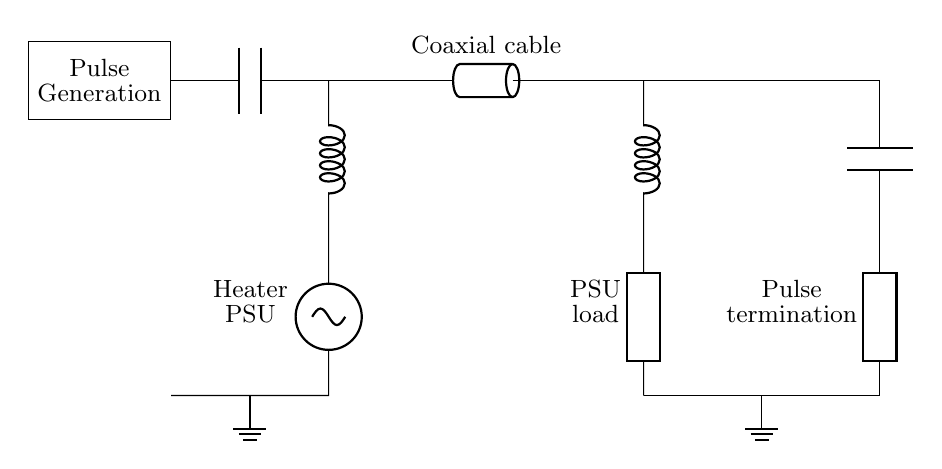
\begin{tikzpicture}

	
	\node (pulse_gen) [rectangle, draw, minimum size=1cm] {\shortstack{Pulse\\Generation}};

	%			to[node, t=\shortstack{Pulse\\Gen.}] ++(1,0)

	%			to[twoport, t=\shortstack{Pulse\\Gen.}] ++(1,0)

	\draw (pulse_gen.east)

	to[C] ++(2,0) coordinate (heater_top);

	
	\draw (heater_top)

	to[L] ++(0,-2)

	to[sV, l_=\shortstack{Heater\\PSU}] ++(0,-2)

	coordinate(heater_btm)

	to[short] ++(-1,0)

	node[ground] {}

	to[short] ++(-1,0);

	
	\draw (heater_top)

	to[TL, l^=Coaxial cable]  ++(4,0)

	coordinate (load_top);

	
	\draw (load_top)

	to[L] ++(0,-2)

	to[R, l_=\shortstack{PSU\\load}] ++(0,-2)

	coordinate(load_btm);

	
	\draw (load_top)

	to[short] ++(3,0)

	coordinate (pulse_term_top);

	
	\draw (pulse_term_top)

	to[C] ++(0,-2)

	to[R, l_=\shortstack{Pulse\\termination}] ++(0,-2)

	coordinate(pulse_term_btm);

	
	\draw (load_btm)

	to[short] ++(1.5,0)

	coordinate[ground]

	to[short] ++(1.5,0);

	
	\end{tikzpicture}

\end{frame}

\begin{frame}{What I've done -- Digital test harness}
	\begin{columns}
	\begin{column}{.49\textwidth}
		\centering
		\begin{tikzpicture}[node distance=\nodeDist,scale=0.45, every node/.style={transform shape}]
		
		\newcommand{\controllerWidth}{4*\blockWidth}
		
		% Controller
		\node (cont) [block, minimum width=\controllerWidth] at (0,0) {\shortstack{Controller}};
		
		% UART RX Stuff
		\node (rx_fifo) [block, above=of cont.north west, anchor=south west] {FIFO};
		\node (msg_asm) [block, above=of rx_fifo.north, anchor=south] {\shortstack{Message\\Assembler}};
		\node (uart_rx) [block, above=of msg_asm.north, anchor=south] {\shortstack{UART\\Receiver}};
		
		\draw [arrowNml] (uart_rx) -- (msg_asm);
		\draw [arrowNml] (msg_asm) -- (rx_fifo);
		\draw [arrowNml] (rx_fifo.south) -- ++(0,-\nodeDist);
		
		% UART TX Stuff
		\node (tx_fifo) [block, above=of cont.north east, anchor=south east] {FIFO};
		\node (msg_disasm) [block, above=of tx_fifo.north, anchor=south] {\shortstack{Message\\Disasembler}};
		\node (uart_tx) [block, above=of msg_disasm.north, anchor=south] {\shortstack{UART\\Transmitter}};
		
		\draw [arrowNml] (msg_disasm) -- (uart_tx);
		\draw [arrowNml] (tx_fifo) -- (msg_disasm);
		\draw [arrowRev] (tx_fifo.south) -- ++(0,-\nodeDist);
		
		%Memory manager
		\node (mem) [block, minimum width=\controllerWidth, below = of cont] {Memory Manager};
		\draw [arrowNml] ([xshift=\blockWidth] cont.south west) -- node[left] {Parameters} ++(0,-\nodeDist);
		\draw [arrowNml] ([xshift=2*\blockWidth] cont.south west) -- node[left] {\shortstack{Replace\\Request}} ++(0,-\nodeDist);
		\draw [arrowRev] ([xshift=3*\blockWidth] cont.south west) -- node[left] {\shortstack{Update}} ++(0,-\nodeDist);
		
		%Demodulatator
		\node (demod) [block, left = of mem] {Demodulator};
		\draw [arrowNml] (cont.west) -| node[above] {Parameters} (demod);
		\draw [arrowNml] (demod) -- (mem);
		\draw [arrowRev] (demod.west) -- node[above] {Input} ++(-1.5*\nodeDist,0);
		
		%Modulatator
		\node (mod) [block, right = of mem] {Modulator};
		\draw [arrowNml] (cont.east) -| node[above] {Parameters} (mod);
		\draw [arrowNml] (mem) -- (mod);
		\draw [arrowNml] (mod.east) -- node[above] {Output} ++(1.5*\nodeDist,0);
		
		
		\end{tikzpicture}
	\end{column}
		
	\begin{column}{.49\textwidth}
		\centering
		\begin{tikzpicture}[node distance=\nodeDist,scale=0.45, every node/.style={transform shape}]
		
		% Clocking
		\node (out_clk) [block] at (0,0) {\shortstack{Output\\Clock\\Generator}};
		\node (bit_ctr) [block, right=of out_clk] {\shortstack{Bit\\Counter}};
		\node (word_ctr) [block, right=of bit_ctr] {\shortstack{Word\\Counter}};
		
		\draw[arrowRev] (out_clk.north) -- ++(0, \nodeDist) node[above] {Parameters};
		\draw[arrowRev] (word_ctr.north) -- ++(0, \nodeDist) node[above] {Parameters};
		
		% Number memory
		\node (num_mem) [block, below = of bit_ctr, minimum width=4*\blockWidth] {Number Memory};
		\draw [arrowRev] (num_mem.west) -- ++(-1.5*\nodeDist,0) coordinate (replace_req) node[left] {\shortstack{Replacement\\request}};
		
		
		%Replacement number shift register
		\node (replace_sr) [block, right = of num_mem.north east, anchor = north west, minimum height= (2*\blockHeight + \nodeDist)] {\shortstack{Replacement\\Number\\Shift\\Register}};
		\draw [arrowNml] (num_mem.east) -- node[above] {\shortstack{Load\\Num.}} ++(\nodeDist, 0);
		
		
		%Received number shift register, and checker
		\node (rec_sr) [block, below = of num_mem.south west, anchor = north west] {\shortstack{Received Number\\Shift Register}};
		\node (checker) [block, below=of num_mem.south east, anchor=north east] {Checker};
		\draw [arrowNml] (checker.south) -- ++(0,-0.5*\nodeDist) node[below] {\shortstack{Incorrect\\Number Received}};
		\draw [arrowNml] (rec_sr) -- node[below] {\shortstack{Parallel\\Out}} (checker);
		\draw [arrowRev] (checker.north) -- node[left] {\shortstack{Expected\\Number}} ++(0,\nodeDist);
		
		%Output Mux
		\node (mux) [block, below=of replace_sr] {Multiplexer};
		\draw[arrowNml] (replace_sr.south) -- node[right] {\shortstack{Shift\\Out}} (mux.north);
		
		\coordinate (in) at ([yshift=-(2*\blockHeight + 2*\nodeDist)]replace_req);
		
		\node[left] at (in) {Input};
		
		\draw [arrowNml] (in) -- ++(0.75*\nodeDist,0) coordinate(input_break) -- (mux);
		
		\draw [arrowNml] (input_break) |- node[left] {Shift in} (rec_sr.west);
		
		\draw [arrowNml] (mux.east) -- ++(1.5*\nodeDist,0) node[right] {Output};
		
		
		\end{tikzpicture}
	\end{column}



	\end{columns}

\end{frame}


\begin{frame}{What I've done -- Test harness software}

\end{frame}

\begin{frame}{What I've done -- System integration}
	\centering
	\includegraphics[height=0.8\textheight]{figs/integrated}
\end{frame}

\begin{frame}{What I've done -- Problems}
	\begin{itemize}
		\item \alert{Many!}
		\item Phantom powering not as simple as first thought
		\item Crosstalk between input and output stages
		\item High speed, high voltage, high power amplifier design
		\item Finding harmony between:
		\begin{itemize}
			\item The literature
			\item What the reconstruction project has made
			\item Very old circuits
			\item Very new circuits
		\end{itemize}
	\end{itemize}
\end{frame}

\begin{frame}{Conclusion}
	\begin{itemize}
		\item \alert{Success!}
		\item What was achieved:
		\begin{itemize}
		\item Analysis of EDSAC's `memory problem'
		\item A working recreation of EDSAC's delay lines that looks and performs as the original (except for phantom power)
		\item A working test harness capable of generating the correct output signals, and analysis of the input signals
		\item A memory system which able to recreate all of the delay line memory in EDSAC, pending careful PCB design and implementation 
		\end{itemize}
	\end{itemize}
\end{frame}

\begin{frame}[standout]
	Demo
\end{frame}

\end{document}